% main.tex

\documentclass[british, 8pt, unknownkeysallowed]{beamer}
% \documentclass[british, 8pt, handout]{beamer} % handout

\usepackage{ragged2e}

% ENCODING AND LANGUAGES : 

%\usepackage{german}
%\usepackage[german,english]{babel}
\usepackage[english]{babel}
% \usepackage[german]
% \usepackage[utf8latin1]{inputenc}
\usepackage[utf8]{inputenc} 


% LOGIC 

\usepackage{forarray}
\usepackage{calc}



% MATH STUFF 
\usepackage{amsmath, amsthm} 
% % % % incompatible to beamer ? 
\usepackage{pxfonts}
\usepackage{pifont}
\usepackage{mathrsfs}
\usepackage{commath}

\usepackage{amsmath} % assumes amsmath package installed
\usepackage{amssymb}  % assumes amsmath package installed
%\usepackage{bm}
\usepackage{mathtools}
% % % 
\theoremstyle{definition}
% \newtheorem{definition}[theorem]{Definition}
\newtheorem{characterization}[theorem]{Characterization}

%% THIS CAN DESTROY A LOT -- DO NOT ACTIVATE THAT ! 
%% \usepackage[charter]{mathdesign}

%% \usepackage[binary,amssymb]{SIunits}%
\usepackage[11pt]{moresize}

% TABLE STUFF 

\usepackage{booktabs}
\usepackage{multirow}
\usepackage{xcolor,colortbl}

\definecolor{Gray}{gray}{0.8}

% GRAPHIX

\usepackage{graphicx}
\usepackage{xcolor}
\usepackage{subfigure}
\usepackage{tikz}
\usepackage{svg}


%
% do not use for beamer since it overwrites the beamer stuff ... , see innertemplate instead ... 
%% \usepackage[figurename=]{caption}

% LAYOUT

\usepackage[overlay,absolute]{textpos}
\usepackage{microtype}


% ALGORITHMS 

\usepackage{listings}


\usepackage{hyperref}

\hypersetup{
    hypertexnames=true,
    unicode     = {false},
    colorlinks  = {false},
    pdftitle    = {},
    pdfsubject  = {},
    pdfauthor   = {},
    pdfkeywords = {},
    pdfborder   = {0 0 0},
    bookmarks   = true,
    breaklinks  = true,
}


% TEMPLATE 

\setbeamersize{text margin left=.33cm,text margin right=.33cm}
% does not have any effect ? 
% \setbeamersize{text margin top=1.5cm, text margin bottom=1.5cm}

% THIS FONT ALSO SCREWS UP THE SPACINGS --> IT NEEDS TO BE PART OF THE TEMPLATE ! 
% IT LOOKS NICER THAN STANDARD FONT ! 
%% 
%% \usepackage{lmodern}
%% 

% tikz needed for beamerthemephbaer
\usepackage{beamer_template_theme_ric_uni_bremen}
\usepackage{tikz}


\beamertemplatenavigationsymbolsempty
\setbeamertemplate{sections/subsections in toc}[circle]
\setbeamercovered{%
  still covered={\opaqueness<1->{20}},
  again covered={\opaqueness<1->{40}}}

\if@twocolumn
  \setlength\leftmargini  {0.7em}
\else
  \setlength\leftmargini  {1.2em}
\fi
\leftmargin  \leftmargini
\setlength\leftmarginii  {1.0em}

% \usepackage{beamer_template_appendixnumber}
\usepackage{appendixnumberbeamer}
% UNSORTED 

\usepackage{textcomp}


\usepackage[backend=biber,sorting=none,style=alphabetic,citestyle=authoryear,maxcitenames=2,maxbibnames=99]{biblatex}
\addbibresource{references.bib}
\AtBeginBibliography{\setcounter{maxnames}{3}}

\newrobustcmd*{\parentexttrack}[1]{%
  \begingroup
  \blx@blxinit
  \blx@setsfcodes
  \blx@bibopenparen#1\blx@bibcloseparen
  \endgroup}

\AtEveryCite{%
  \let\parentext=\parentexttrack%
  \let\bibopenparen=\bibopenbracket%
  \let\bibcloseparen=\bibclosebracket}


% define bib item template with larger graphic
\defbeamertemplate{bibliography item}{mybibitem}
{\textbullet} % \lower5pt\hbox{\scalebox{2}{}}} % \pgfuseimage{beamericonarticle}

% choose to show enlarged article items using that template
% \setbeamertemplate{bibliography item}[mybibitem]
\setbeamertemplate{bibliography item}[text]
 
 
% text_maccros

\newcommand{\inputTheSmallFigure}[1]
{\raisebox{-0.25cm}{\includegraphics[width=0.8cm]{figures/math/quaternions/coords/#1}}}
 
\newcommand{\yepp}{\ding{51}}
\newcommand{\nope}{\text{--}}

% \newcommand{\CadToSim}{\texttt{CAD-2-SIM}}


\newcommand{\isf}[1]{\inputTheSmallFigure{#1}}

% \inputSmallMatrix
\newcommand{\ism}[9]{$\biggl[\begin{smallmatrix}#1&#2&#3\\#4&#5&#6\\#7&#8&#9\end{smallmatrix}\biggr]$}

% % % 
\newcommand{\smallhyperlink}[2]     {{\small\href{#1}{#2}}}
\newcommand{\sepsmallhyperlink}[2]  {\begin{itemize}\item \smallhyperlink{#1} \end{itemize}}
% % % 
% % % 
\newcommand{\smallurl}[1]     {{\tiny\url{#1}}}
\newcommand{\sepsmallurl}[1]  {\begin{itemize}\item \smallurl{#1} \end{itemize}}
% quotation marks - G erman :
\newcommand{\glr}{bla}
\newcommand{\gqq}[1]{\glqq #1\grqq}
\newcommand{\gq}[1] {\glq  #1\grq}
% quotation marks - E nglish : 
\newcommand{\eqq}[1]{\lq\lq #1\rq\rq}
\newcommand{\eq}[1] {\lq  #1\rq}
% quotation marks - F rench : 
\newcommand{\fqq}[1]{\flqq #1\frqq}
\newcommand{\fq}[1] {\flq #1\frq}

% write something like >@somebody< with the commmand >\at somebody<
\newcommand{\at}{$@$}


\newcommand{\req}[1]    {Equation~\ref{#1}}
\newcommand{\rseq}[1]   {Eq.~\ref{#1}}

\newcommand{\rsec}[1]   {Section~\ref{#1}}
\newcommand{\rfig}[1]   {Figure~\ref{#1}}
\newcommand{\rdiag}[1]  {Diagram~\ref{#1}}
\newcommand{\rpar}[1]   {Paragraph~\ref{#1}}
\newcommand{\rtab}[1]   {Table~\ref{#1}}
\newcommand{\rapp}[1]   {Appendix~\ref{#1}}
\newcommand{\rexa}[1]   {Example~\ref{#1}}


% % todo A NICE FEATURE to MARK development directives: 
\newcommand{\temptext}[1]{\noindent\fcolorbox{lightgray}{white}{\color{gray}\begin{minipage}{\textwidth}{#1}\end{minipage}}\color{black}}


\newcommand{\technical}[1]{\texttt{#1}}

% A
\newcommand{\ADRF}{\technical{ADRF}}
\newcommand{\AutodeskInventor}{\technical{Autodesk Inventor}}
% C
\newcommand{\CAD}{\technical{CAD}}
\newcommand{\CadToSim}{\technical{CAD-2-SIM}} 
\newcommand{\cpp}{\technical{C++}}
\newcommand{\Cpp}{\technical{C++}}
% G 
\newcommand{\GUI}{\technical{GUI}}
% L 
\newcommand{\Latex}{\technical{\LaTeX}}
% M 
\newcommand{\Mars}{\technical{Mars}}
\newcommand{\Matlab}{\technical{Matlab}}
% O 
\newcommand{\Openrave}{\technical{Openrave}}
\newcommand{\opensim}{\technical{OpenSim}}
% P
\newcommand{\Python}{\technical{Python}}
\newcommand{\python}{\technical{Python}}


% S 
\newcommand{\Simulink}{\technical{Simulink}}
\newcommand{\Solidworks}{\technical{SolidWorks}}
\newcommand{\SolidWorks}{\technical{SolidWorks}}
\newcommand{\simtk}{\technical{SimTK}}
\newcommand{\simbody}{\technical{SimBody}}
% V 
\newcommand{\Visualbasic}{\technical{VisualBasic}}
% W
\newcommand{\WRL}{\technical{WRL}}
% X
\newcommand{\XML}{\technical{XML}} 



% slide_macros

\newcommand{\separationframe}[1]{\frame[noframenumbering]{\structpartshort{#1}}}



% \newcommand{\specialSeparationframe}[2]{%
% \frame{\begin{center}%
% \includegraphics[width=0.66\linewidth]{#2}%                                                 
% \end{center}% 
% \vspace*{0.1cm}
% {\color{capiogray}\huge #1}}
% }

\newcommand{\specialSeparationframe}[2]{%
\begin{frame}
% \pgfputat{\pgfxy(10.5, 2.5)}{\pgfbox[left,top]{\includegraphics[width=0.66\linewidth]{#2}}}
% \pgfputat{\pgfxy(10.5, 5.5)}{\pgfbox[left,top]{\includegraphics[height=1cm]{figures/cad_2_sim_logo}}}
% \pgfputat{\pgfxy(1.0, 5.5)}{\pgfbox[left,top]{\color{capiogray}\huge #1}}}
% \pgfputat{\pgfxy(1.0, 5.5)}{\pgfbox[left,top]{\color{capiogray}\huge #1}} 
% 
\begin{center}
\begin{columns}[c]
\begin{column}{0.15\linewidth}
 
\end{column}

\begin{column}{0.35\linewidth}
  \scriptsize 
  \tableofcontents[currentsection]
\end{column}

\begin{column}{0.48\linewidth}
\includegraphics[width=0.99\linewidth]{#2}
\end{column}
% 
\end{columns}
\end{center}

{\color{capiogray}\huge #1}
% 

\end{frame}
}


%% {\color{fg!35}bla}

% % % \usepackage{paralist}
% % % 
% % % \setlength{\pltopsep}       {2pt}       % Space between first item and preceding paragraph.
% % % \setlength{\plpartopsep}    {0pt}       % Extra space added to \topsep when environment starts a new paragraph (is called in vmode).
% % % 
% % % \setlength{\plitemsep}      {0pt}       % Space between successive items.
% % % \setlength{\plparsep}       {0pt}       % Space between paragraphs within an item – the \parskip for this environment.
% % % 
% % % \newenvironment{itemizeflat}
% % % {\begin{compactitem}}
% % % {\end{compactitem}}
% % % 
% % % \newenvironment{enumerateflat}
% % % {\begin{compactenum}}
% % % {\end{compactenum}}


\newcommand{\pim}{\pause \item}

\newcommand{\bluemph}[1]{\textcolor{blue}{#1}}


% centering an image (needed for background image) -- three arguments 
% 
%   #1  --  figure width
%   #2  --  figure vertical offset 
%   #3  --  the figure file 
% 
\newcommand{\centergraphics}[3]
{
\parbox[c]{\paperwidth}{\vspace*{#2\paperwidth}\centering\includegraphics[width=#1\linewidth]{#3}}
}


% making an image opaque (nice for background images) -- four arguments 
% 
%   #1  --  opacity value 
%   #2  --  figure width
%   #3  --  figure vertical offset 
%   #4  --  the figure file 
% 
\newcommand{\opaccentergraphics}[4]
{
\tikz\node[opacity=#1]{\centergraphics{#2}{#3}{#4}};
}


% centralize anything easily ... with restricted width 
% 
\newenvironment{slimcenter}[1]
{%
  \begin{columns}\begin{column}{#1}
}{%
  \end{column}\end{columns}
}


% centralize figure easily ... 
% 
\newenvironment{figureH}
{% 
  \begin{figure}[H]\centering
}% 
{% 
  \end{figure}
}

% centralize table easily ... 
% 
\newenvironment{tableH}
{% 
  \begin{table}[H]\centering
}% 
{% 
  \end{table}
}


% tweaking the quote environment 
% 
\renewenvironment{quote}
  {\list{}{\leftmargin=0.3cm\rightmargin=0.3cm}\item[]\color{capiogray}\it}
  {\endlist}

% giving the source for a quotation 
% 
\newcommand{\quotesource}[1]
  {\hspace*{\fill}\textup{\color{black}#1}}


% --------------------------------------------------------------------------------

% 
% TODO : FOR CUSTOM BOXES -- check 'tcolorbox' -- see http://tex.stackexchange.com/questions/27093/what-are-alternatives-to-block
% 

% --------------------------------------------------------------------------------

% an environment to refer too publications 
% 
\newenvironment<>{slideBibBox}
{%
    \begin{actionenv}%
    \def\insertblocktitle{\footnotesize{Publication}}%
    \par%
     \mode<presentation>{%
        % \setbeamercolor{block title}{ fg=white,bg=orange!20!black}
        % \setbeamercolor{block body}{fg=black,bg=olive!50}
        % \setbeamercolor{itemize item}{fg=orange!20!black}
        % \setbeamertemplate{itemize item}[triangle]
     }%
    \usebeamertemplate{block begin}\footnotesize}
{
    \par\usebeamertemplate{block end}
    \end{actionenv}
}

\newcommand{\currentPubState}[1]    {({\texttt{\tiny#1}})}

\newcommand{\bibWHO}[1]     {#1.\ }
\newcommand{\bibWHAT}[1]    {\emph{\eqq{#1}}.\ }
\newcommand{\bibWHERE}[1]   {#1,\ }
\newcommand{\bibWHEN}[1]    {#1.\ }
\newcommand{\bibSTATUS}[1]  {\currentPubState{#1}}

\newcommand{\bibWhoWhatWhereWhenStatus}[5]  
{% 
    \bibWHO{#1}\bibWHAT{#2}\bibWHERE{#3}\bibWHEN{#4}\bibSTATUS{#5}% 
}% 

\newcommand{\bibWhoWhatWhereWhenPublished}[4]  
{% 
    \bibWHO{#1}\bibWHAT{#2}\bibWHERE{#3}\bibWHEN{#4}% 
}% 

% --------------------------------------------------------------------------------


% an environment to refer too publications 
% 
\newenvironment<>{slideWhitePaperBox}
{%
    \begin{actionenv}%
    \def\insertblocktitle{\footnotesize{Whitepaper}}%
    \par%
     \mode<presentation>{%
        % \setbeamercolor{block title}{ fg=white,bg=orange!20!black}
        % \setbeamercolor{block body}{fg=black,bg=olive!50}
        % \setbeamercolor{itemize item}{fg=orange!20!black}
        % \setbeamertemplate{itemize item}[triangle]
     }%
    \usebeamertemplate{block begin}\footnotesize}
{
    \par\usebeamertemplate{block end}
    \end{actionenv}
}

% --------------------------------------------------------------------------------

\newcommand{\whiteWhat}[1]     {\emph{\eq{#1}}.}

% --------------------------------------------------------------------------------


% some general purpose math macros 
% 



%
% some commands for including four figures into one slide ... 
% 


% a maximal figure - see http://tex.stackexchange.com/questions/32886/how-to-fit-a-large-figure-to-page
% 
\newcommand{\ingraphmax}[1] 
{
  {
    \setlength{\fboxsep}{0pt}     %padding thickness
    \setlength{\fboxrule}{1pt}    %padding thickness
    \centering 
    % 
    \newpage\fcolorbox{lightgray}{white}{\includegraphics[width=\textwidth,height=\textheight,keepaspectratio]{#1}}
  }
}

% 'ingraph' -- shorter proxy for 'includegraphics'
% 
\newcommand{\ingraph}[2]{
  \centering\includegraphics[width=#1\linewidth]{#2}
}


\newcommand{\fourFigureGraphics}[1]     {\centering\includegraphics[width=0.8\linewidth]{#1}}

\newcommand{\fourFigureFrame}[5]    
{\begin{frame}{#1}
% 
\vspace*{0.05cm}
\begin{columns}
\centering 
\begin{column}[t]{0.49\linewidth}
\fourFigureGraphics{#2}
\end{column}
\quad 
\begin{column}[t]{0.49\linewidth}
\fourFigureGraphics{#3}
\end{column}
\end{columns}
\vspace*{0.25cm}
\begin{columns}
\centering 
\begin{column}[t]{0.49\linewidth}
\fourFigureGraphics{#4}
\end{column}
\quad 
\begin{column}[t]{0.49\linewidth}
\fourFigureGraphics{#5}
\end{column}
\end{columns}
% 
\end{frame}
}


\newcommand{\fourFigureFramePaused}[5]    
{\begin{frame}{#1}
% 
\vspace*{0.05cm}
\begin{columns}
\centering 
\begin{column}[t]{0.49\linewidth}
% \visible<2->
{\fourFigureGraphics{#2}}
\end{column}
\quad 
\begin{column}[t]{0.49\linewidth}
% \visible<3->
{\fourFigureGraphics{#3}}
\end{column}
\end{columns}
\vspace*{0.25cm}
\begin{columns}
\centering 
\begin{column}[t]{0.49\linewidth}
% \visible<4->
{\fourFigureGraphics{#4}}
\end{column}
\quad 
\begin{column}[t]{0.49\linewidth}
% \visible<5->
{\fourFigureGraphics{#5}}
\end{column}
\end{columns}
% 
\end{frame}
}


\newcommand{\twoFigureFrame}[3]  
{\begin{frame}{#1}
% 
\begin{columns}
\centering 
\begin{column}[t]{0.49\linewidth}
\ingraphmax{#2}
\end{column}
\quad 
\begin{column}[t]{0.49\linewidth}
\ingraphmax{#3}
\end{column}
\end{columns}
% 
\end{frame}
}



\newcommand{\twoFigureFramePaused}[3]  
{\begin{frame}{#1}
% 
\begin{columns}
\centering 
\begin{column}[t]{0.49\linewidth}
% \visible<2->
{\ingraphmax{#2}}
\end{column}
\quad 
\begin{column}[t]{0.49\linewidth}
% \visible<3->
{\ingraphmax{#3}}
\end{column}
\end{columns}
% 
\end{frame}
}


% THIS CAN BE DANGEROUS together with indexing ! 
% 
% active  short verbatim environment between vertical bars a la '|a verb expression|'
% 
\usepackage{fancyvrb}
% 
% this one creates conflicts with makeindex: 
% \DefineShortVerb{\|}
% 
% this one DOES NOT create conflicts with glossaries (at least with texlive 2012): 
\DefineShortVerb{\"}


% -----------------------------------------


\usepackage{relsize}


% -----------------------------------------


% -----------------------------------------


% a flat fraction
% 
\newcommand{\flatfrac}[2]{\ensuremath{#1\,/\,#2}}

% a small fraction
% 
\newcommand{\smallfrac}[2]{\text{\scriptsize$\frac{#1}{{#2}}$}}


\usepackage{fancybox}
\newcommand{\someBox}[1]        {\Ovalbox{#1}}

% -----------------------------------------

\usepackage{lmodern}
% \usefonttheme{serif}


\newcommand{\hdffive}    {\texttt{HDF5}}
\newcommand{\yaml}       {\texttt{Yaml}}



% % some general purpose math macros 
% 

\input{defines/mathematics/variables_and_constants}
\input{defines/mathematics/environments}
% \input{defines/mathematics/macros}


% some document specific math macros 


% -----------------------------------------


% \newcommand{\medfrac}   [2] {\mathsmaller{\frac{#1}{#2}}}


\setbeamercovered{invisible}
% \setbeamercovered{transparent} 
% \newcommand{\stdvec}    [1]             {\vect{\hat{e}}\losmall{#1}} % \hismall{(#1)}}}


\newenvironment<>{tempbox}[1][]{%
  \setbeamercolor{block title example}{fg=white,bg=red!75!black}%
  \begin{block}{}\ttfamily}
{\end{block}}

\newenvironment<>{blockquestion}[1][]{%
  \setbeamercolor{block title}{fg=white,bg=red!50!black}%
  \begin{block}{Question}}
{\end{block}}

\newenvironment<>{blockexample}[1][]{%
  % \setbeamercolor{block title}{fg=white,bg=red!50!black}%
  \begin{example}[#1]}
{\end{example}}


\newenvironment<>{blockcharacterization}[1][]{%
  \setbeamercolor{block title}{fg=white,bg=blue!15!gray}%
  \begin{block}{Characterization (#1)}}
{\end{block}}



\newenvironment<>{blockredefinition}[1][]{%
    \setbeamercolor{block title}{fg=white,bg=red!50!black}%
  \begin{block}{Redefinition (#1)}}
{\end{block}}


\newenvironment<>{blockstructure}[1][]{%
  % \setbeamercolor{block title}{fg=white,bg=red!50!black}%
  \begin{block}{Structure}}
{\end{block}}





% adaptable alternative to 
%   \footfullcite{2002_book_Kuipers_Quaternions}
% reads 
% 

\newcommand\blfootnote[1]{%
  \begingroup
  \renewcommand\thefootnote{}\footnote{#1}%
  \addtocounter{footnote}{-1}%
  \endgroup
}

\newcommand{\printpublication}[1]{\AtNextCite{\defcounter{maxnames}{99}}\fullcite{#1}}

\newcommand{\footcitenice}      [1] {\blfootnote{\tiny \printpublication{#1}}}
\newcommand{\footcitesnice}     [2] {\blfootnote{\textsf{\tiny \printpublication{#1},\printpublication{#2}}}}
\newcommand{\footcitenicenumber}      [1] {\footnote{\tiny \printpublication{#1}}}
\newcommand{\footcitesnicenumber}     [2] {\footnote{\textsf{\tiny \printpublication{#1},\printpublication{#2}}}}
\newcommand{\parencitesmall}      [1] {{\small \parencite{#1}}}
\newcommand{\parencitetiny}      [1] {{\tiny \parencite{#1}}}


\setbeameroption{show notes}
\setbeamertemplate{note page}[plain]


\usepackage{tikz}



% http://tex.stackexchange.com/questions/86188/labelling-with-arrows-in-an-automated-way
% 
% formula, text, node#
% % \newcommand{\mathWithDescription}[3]{%
% % \tikz[baseline]{%
% %     \node[draw=red,rounded corners,anchor=base] (m#3)%
% %     {$\displaystyle#1$};%
% %     \node[above of=m#3] (l#3) {#2};%
% %     \draw[-,red] (l#3) -- (m#3);%
% % }%
% % }


\newcommand{\mathWithDescription}[3]{%
\tikz[baseline]{%
    \node[draw=red,rounded corners,anchor=base] (m#3)%
    {$\displaystyle#1$};%
    \node[below of=m#3] (l#3) {#2};%
    \draw[-,red] (l#3) -- (m#3);%
}%
}


\newcounter{mathLableNode}

\newcommand{\mathLabelBox}[2]{%
   \stepcounter{mathLableNode}%
   \mathWithDescription{#1}{#2}{\themathLableNode}%
}

\newcommand{\boxedRED}[1]{%
\tikz[baseline]{\node[draw=red,rounded corners,anchor=base] (m){\ensuremath{#1}};}
}

% set verbatim to tiny 
% 
\makeatletter
\def\verbatim@font{\ttfamily\tiny}
\makeatother


% defining some math commands 
% 
% \newcommand{\COMMANDNAME}  [NOARGS] {\boldsymbol{REFARGINDEX}}  
% 
\newcommand{\vect}      [1] {\boldsymbol{#1}}
\newcommand{\mat}       [1] {\boldsymbol{#1}}
\newcommand{\tEXP}          {^{\mathsmaller{T}}}
\newcommand{\losmall}   [1] {_{\mathsmaller{#1}}}
\DeclareMathOperator*{\argmin}{arg\,min}

\newcommand{\chapquote}[3]{\begin{quotation} \textit{#1} \end{quotation} \begin{flushright} -- #2, \textit{#3}\end{flushright} }
% some macros ... 
% 
\newcommand{\keypoint}  [1]     {\bluemph{\emph{#1}}}

\newcommand{\KEYsubmechanism}      {\keypoint{Submechs}}
\newcommand{\KEYpersons}           {\keypoint{Persons}} 
\newcommand{\KEYmethods}           {\keypoint{Methods}} 
\newcommand{\KEYimplementation}    {\keypoint{Implementation}}
\newcommand{\KEYlinks}             {\keypoint{Links}} 


% for defining new columntypes 
% 
\usepackage{array}


% cite title and year 
% 
\newcommand{\citeTY}    [1]         {\emph{\citetitle{#1}, \citeyear{#1}}}
\newcommand{\citeATY}   [1]         {\emph{\citeauthor{#1},
\citetitle{#1}, \citeyear{#1}}}

\newcommand{\highlight}[1]{%
  \colorbox{red!50}{$\displaystyle#1$}}

% ------------------------------------------------------------------------------------------------------------------------------------------
% --> all three 
% ------------------------------------------------------------------------------------------------------------------------------------------

\usepackage[printonlyused]{acronym}
\usepackage{multimedia}
\usepackage[normalem]{ulem}
% \usepackage{enumitem}
\usepackage[multiple,flushmargin,hang]{footmisc}

% ------------------------------------------------------------------------------------------------------------------------------------------
% --> all three 
% ------------------------------------------------------------------------------------------------------------------------------------------

\beamertemplatenavigationsymbolsempty
\setbeamertemplate{sections/subsections in toc}[circle]
\setbeamercovered{%
  still covered={\opaqueness<1->{0}},
  again covered={\opaqueness<1->{40}}}
  
\let\oldfootnote\footnote
\renewcommand\footnote[1][]{\oldfootnote[frame,#1]}  
\addtobeamertemplate{footnote}{}{\vspace{2ex}}

\usepackage{xpatch}% or use http://tex.stackexchange.com/a/40705

\def\makenamesetup{%
  \def\bibnamedelima{~}%
  \def\bibnamedelimb{ }%
  \def\bibnamedelimc{ }%
  \def\bibnamedelimd{ }%
  \def\bibnamedelimi{ }%
  \def\bibinitperiod{.}%
  \def\bibinitdelim{~}%
  \def\bibinithyphendelim{.-}}    
\newcommand*{\makename}[3]{\begingroup\makenamesetup\xdef#1{#2, #3}\endgroup}

\newbibmacro*{name:bold}[2]{%
  \makename{\currname}{#1}{#2}%
  \makename{\findname}{\lastname}{\firstname}%
  \makename{\findinit}{\lastname}{\firstinit}%
  \ifboolexpr{ test {\ifdefequal{\currname}{\findname}}
            or test {\ifdefequal{\currname}{\findinit}} }{\bfseries}{}}

\newcommand*{\boldname}[3]{%
  \def\lastname{#1}%
  \def\firstname{#2}%
  \def\firstinit{#3}}
\boldname{}{}{}

\xpretobibmacro{name:last}{\begingroup\usebibmacro{name:bold}{#1}{#2}}{}{}
\xpretobibmacro{name:first-last}{\begingroup\usebibmacro{name:bold}{#1}{#2}}{}{}
\xpretobibmacro{name:last-first}{\begingroup\usebibmacro{name:bold}{#1}{#2}}{}{}
\xpretobibmacro{name:delim}{\begingroup\normalfont}{}{}

\xapptobibmacro{name:last}{\endgroup}{}{}
\xapptobibmacro{name:first-last}{\endgroup}{}{}
\xapptobibmacro{name:last-first}{\endgroup}{}{}
\xapptobibmacro{name:delim}{\endgroup}{}{}

% just for demonstration
%\ExecuteBibliographyOptions{maxnames=99,firstinits}
%\DeclareNameAlias{default}{last-first/first-last}
%
%\boldname{W{\"o}hrle}{Hendrik}{H.}
%\boldname{Woehrle}{Hendrik}{H.}

\begin{document}
\newcommand{\robotName}{RH5V2}

%%%%%%%%%%%%%%%%%%%%%%%%%%%%%%%%%%%%%%%%%
\newcommand{\mvec}[1]{\bm{#1}}
\newcommand{\vc}[1]{\mathbf{\mathbf{#1}}}
%%%%%%%%%%%%%%%%%%%%%%%%%%%%%%%%%%%%%%%%%

\newcommand{\q}{\textbf{q}}
\newcommand{\dq}{\dot{\q}}
\newcommand{\ddq}{\ddot{\q}}

%%%%%%%%%%%%%%%%%%%%%%%%%%%%%%%%%%%%%%%

\newcommand{\Mass}{\mathbf{M}}
\newcommand{\Bias}{\mathbf{b}}
\newcommand{\Gravity}{\mathbf{g}}
\newcommand{\Force}{\mathbf{\lambda}}
\newcommand{\Torque}{\mathbf{\tau}}
\newcommand{\Jac}{\mathbf{J}}

%%%%%%%%%%%%%%%%%%%%%%%%%%%%%%%%%%%%%%%%%
\newcommand{\BIN}{\begin{bmatrix}}
\newcommand{\BOUT}{\end{bmatrix}}

%%%%%%%%%%%%%%%%%%%%%%%%%%%%%%%%%%%%%%%%%
\newcommand{\sref}[1]{Sec~\ref{#1}}
\newcommand{\eref}[1]{(\ref{#1})}
\newcommand{\fref}[1]{Fig.~\ref{#1}}
\newcommand{\tref}[1]{Table~\ref{#1}}

%%%%%%%%%%%%%%%%%%%%%%%%%%%%%%%%%%%%%%%%
\newcommand{\state}{\mathbf{x}}
\newcommand{\ctrl}{\mathbf{u}}
\newcommand{\dynsys}{\mathbf{f}}


%%%%%%%%%%%%%%%%%%%%%%%%%%%%%%%%%%%%%%%
\newcommand{\qTr}{\underline{\q}}
\newcommand{\dqTr}{\underline{\dq}}
\newcommand{\ddqTr}{\underline{\ddq}}
\newcommand{\TorqueTr}{\underline{\Torque}}

%%%%%%%%%%%%%%%%%%%%%%%%%%%%%%%%%%%%%%
\newcommand{\costl}{l}
\newcommand{\dts}{\Delta t_s}
\newcommand{\st}{\text{subject to}}

%\boldname{W{\"o}hrle}{Hendrik}{H.}
%\boldname{Woehrle}{Hendrik}{H.}



% ------------------------------------------------------------------------------------------------------------------------------------------
% --> all three 
% ------------------------------------------------------------------------------------------------------------------------------------------



\title   {Robust Co-design for Underactuated Systems}
\subtitle {Master thesis exposé}
\author   [Federico Girlanda]{BSc Federico Girlanda}
\date     [2022-09]{September, 28th 2022}
\institute[DFKI Bremen]{DFKI Robotics Innovation Center Bremen}


%%%%%%%%%%%%%%%%%%%%%%%%%%%%%%%%%%%%%%%%%%%%%%%%%%%%%%%%%%%%%%%%%%%%%%%%%%%% 

% \begingroup
% \setbeamertemplate{footline}{}
% \frame{\titlepage
% }
% \endgroup

\begin{frame}
 \maketitle
\end{frame}

\begin{frame}{About Me}
\begin{columns}
\begin{column}{\linewidth}
\begin{block}{Background}
\begin{minipage}{.7\linewidth}
\begin{itemize}
  \item Coming from: Verona, Italy
  \item University: University of Padua
  \item Previous studies: Bachelor degree in Electrical Engineering
  \item Current studies: Master degree in Control Systems Engineering
  \item 03/2022: Start of my DFKI experience
\end{itemize}
\end{minipage}
\begin{minipage}{.2\linewidth}
\raggedleft
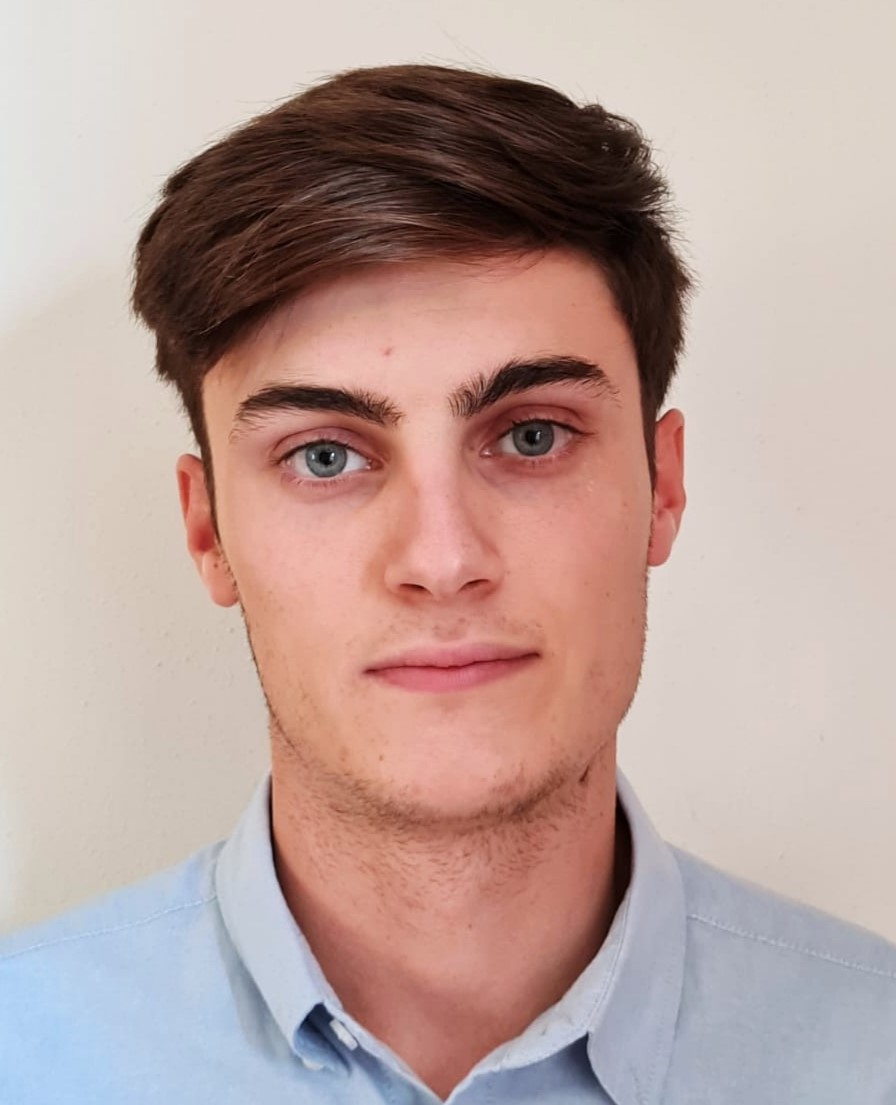
\includegraphics[width=0.6\linewidth, height = 0.7\linewidth]{figures/cvPhoto.jpg}
\end{minipage}
\end{block}
\begin{block}{Motivational quote}
\centering
''I have grown a deep interest in the fields of robotics and automation during my studies.\\
Now is the moment to put into practise all these academic knowledge!''
\end{block}
\end{column}
\end{columns}
\end{frame}

% \subsection*{Table of Content}
\begin{frame}{Table of Content}
\tableofcontents
\end{frame}

%%%%%%%%%%%%%%%%%%%%%%%%%%%%%%%%%%%%%%%%%%%%%%%%%%%%%%%%%%%%%%%%%%%%%%%%%%%%

\section{Introduction}
\separationframe{Introduction}

\begin{frame}{Extreme Athletic Intelligence}
\centering
\movie[autostart, loop, width=0.45\textwidth, height = 0.58\textwidth, showcontrols]{}{figures/boltRun.mp4}
\movie[autostart, loop, width=0.45\textwidth, height = 0.58\textwidth, showcontrols]{}{figures/phelpsSwim.mp4}
\end{frame}

\begin{frame}{Trajectory Optimization}
\begin{minipage}{.45\linewidth}
\centering
\begin{block}{Training: knowing how to run}
\begin{itemize}
\item Breath managing
\item Keeping focus
\item How to deal with curves
\end{itemize}
\end{block}
\end{minipage}
\begin{minipage}{.45\linewidth}
\centering
\begin{figure}
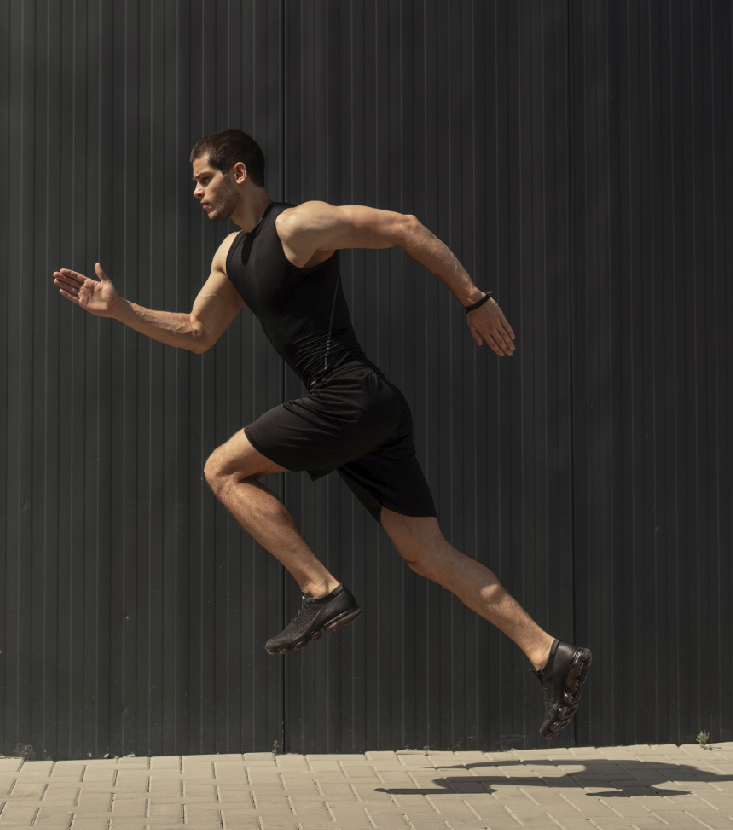
\includegraphics[width=0.6\linewidth, height=0.8\linewidth]{figures/humanRun.png}
\caption{Figure 1: running man}
\end{figure}
\end{minipage}
\end{frame}

\begin{frame}{Design Optimization}
\begin{minipage}{.45\linewidth}
\centering
\begin{block}{Physical characteristics}
\begin{itemize}
\item Body weight
\item Leg length
\item Muscles
\end{itemize}
\end{block}
\end{minipage}
\begin{minipage}{.45\linewidth}
\centering
\begin{figure}
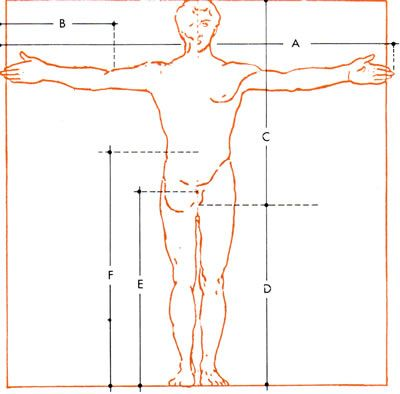
\includegraphics[width=0.6\linewidth, height=0.6\linewidth]{figures/humanDesign.jpg}
\caption{Figure 2: human body measures}
\end{figure}
\end{minipage}
\end{frame}

\begin{frame}{Trajectory Stabilization}
\begin{minipage}{.45\linewidth}
\centering
\begin{block}{Non-ideal conditions}
\begin{itemize}
\item How to face different ground surfaces
\item How to deal with different weather conditions
\end{itemize}
\end{block}
\end{minipage}
\begin{minipage}{.45\linewidth}
\centering
\begin{figure}
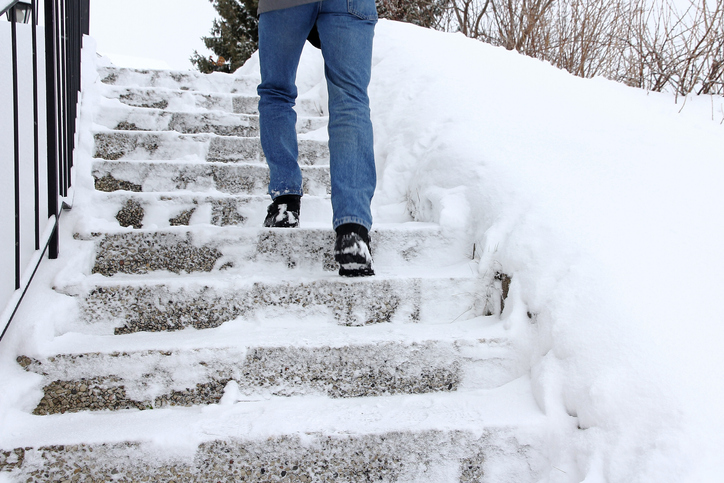
\includegraphics[width=0.6\linewidth, height=0.7\linewidth]{figures/slipGround.jpg}
\caption{Figure 3: slippery ground}
\end{figure}
\end{minipage}
\end{frame}

\begin{frame}{The Optimal Interplay}
\centering
\begin{figure}
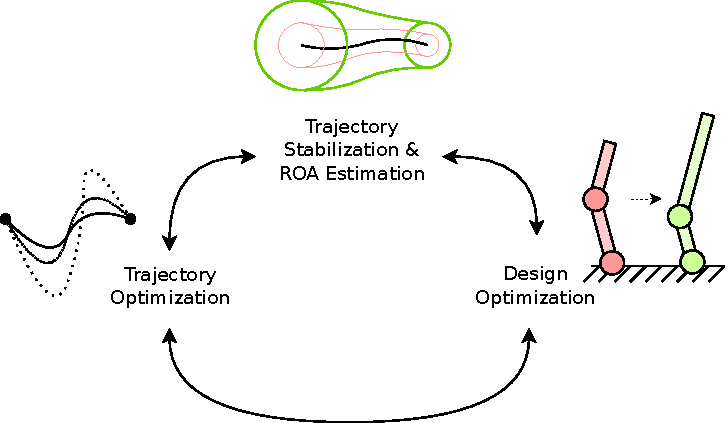
\includegraphics[width=0.8\linewidth, height=0.45\linewidth]{figures/interplay.pdf}
\caption{Figure 4: interplay between different kind of optimization}
\end{figure}
\end{frame}

\section{State of the Art and Objectives}
\separationframe{State of the Art and Objectives}

\begin{frame}{Co-design}
\begin{minipage}{.2\linewidth}
\centering
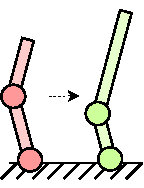
\includegraphics[width=0.6\linewidth, height = 0.7\linewidth]{figures/desOpt.pdf}
\vspace{1cm}\\
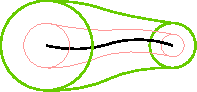
\includegraphics[width=0.6\linewidth, height = 0.5\linewidth]{figures/trajStab.pdf}\\
\vspace{0.8cm}
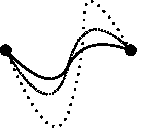
\includegraphics[width=0.6\linewidth, height = 0.6\linewidth]{figures/trajOpt.pdf}\\
\end{minipage}
\begin{minipage}{.1\linewidth}
\raggedright

\includegraphics[width=0.6\linewidth, height = 1.3\linewidth]{figures/doubleArrow.pdf}\\
\vspace{1cm}

\includegraphics[width=0.6\linewidth, height = 1.3\linewidth]{figures/doubleArrow.pdf}\\
\end{minipage}
\begin{minipage}{.6\linewidth}
\begin{block}{}
\begin{itemize}
  \item 2007: Length ratio optimization in Acrobot design $^{\left[1\right]}$
  \item 2022: Robust co-optimization of Acrobot design and controller for up-right stabilization $^{\left[2\right]}$
\end{itemize}
\end{block}
\vspace{0.5cm} 
\begin{block}{}
\begin{itemize}
  \item 2017: DIRTREL, robust trajectory optimization with ellipsoidal disturbances and LQR feedback $^{\left[3\right]}$
  \item 2020: Progress on Atlas, the world's most dynamic humanoid robot $^{\left[4\right], \left[5\right]}$
\end{itemize}
\end{block}
\end{minipage}
\vspace{0.1cm} 
\end{frame}

\begin{frame}{RoA Estimation}
\begin{minipage}{.3\linewidth}
\centering
\vspace{0.3cm}
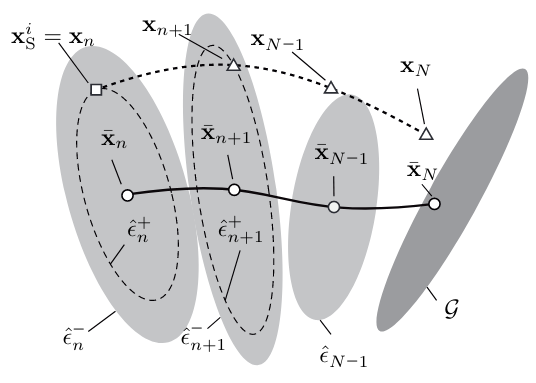
\includegraphics[width=0.6\linewidth, height = 0.45\linewidth]{figures/ReistSbEstMethod.png}\\
\vspace{1.4cm}
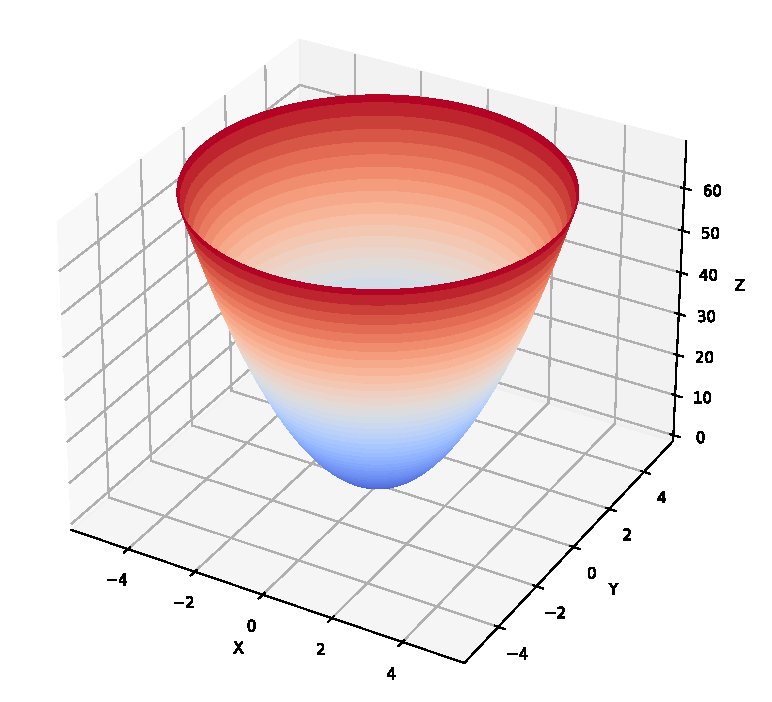
\includegraphics[width=0.6\linewidth, height = 0.6\linewidth]{figures/paraboloid.pdf}\\
\end{minipage}
\begin{minipage}{.6\linewidth}
\begin{block}{}
\begin{itemize}
  \item 2016: A fast sampling method for estimating the time invariant domain of attraction $^{\left[6\right]}$
  \item 2016: Simulation-based estimation method for time varying RoA $^{\left[7\right]}$
\end{itemize}
\end{block}
\vspace{0.5cm}
\begin{block}{}
\begin{itemize}
  \item 2010: Time varying RoA estimation using sum-of-squares programming $^{\left[8\right]}$
  \item 2012: Acrobot robust control design along trajectories with sums of squares programming $^{\left[9\right]}$
  \item 2014: Robust post-stall perching with a simple fixed-wing glider using LQR-Trees $^{\left[10\right]}$
\end{itemize}
\end{block}
\end{minipage}
\end{frame}

\begin{frame}{The Challenge}
\begin{block}{Main goals}
\begin{itemize}
\item Time-varying RoA estimation for Acrobot with sum-of-squares programming
\item Robust interplay between trajectory stabilization and design optimization
\item Combined controller and design optimization for robustness along trajectories
\end{itemize}
\end{block}
\begin{block}{Stretched objectives}
\begin{itemize}
\item Robust interplay between trajectory stabilization and trajectory optimization
\item Full co-design algorithm for best performances and robustness
\end{itemize}
\end{block}
\end{frame}

\section{Region of Attraction Estimation}
\separationframe{Region of Attraction Estimation}

\begin{frame}{The Pendulum Dynamics: EOM}
\begin{block}{State space equations}
\begin{minipage}{.4\linewidth}
\[x = \begin{bmatrix}\theta \\ \dot{\theta}\end{bmatrix}\]
\end{minipage}
\begin{minipage}{.4\linewidth}
\[\dot{x} = \begin{bmatrix}\dot{\theta}\\ \frac{\tau_{in}}{m L^2} - \frac{g}{L} sin(\theta) - \frac{b}{m} \dot{\theta}\end{bmatrix}\]
\end{minipage}
\end{block}
\begin{figure}[!h] 
\centering
\vspace{0.5 cm}
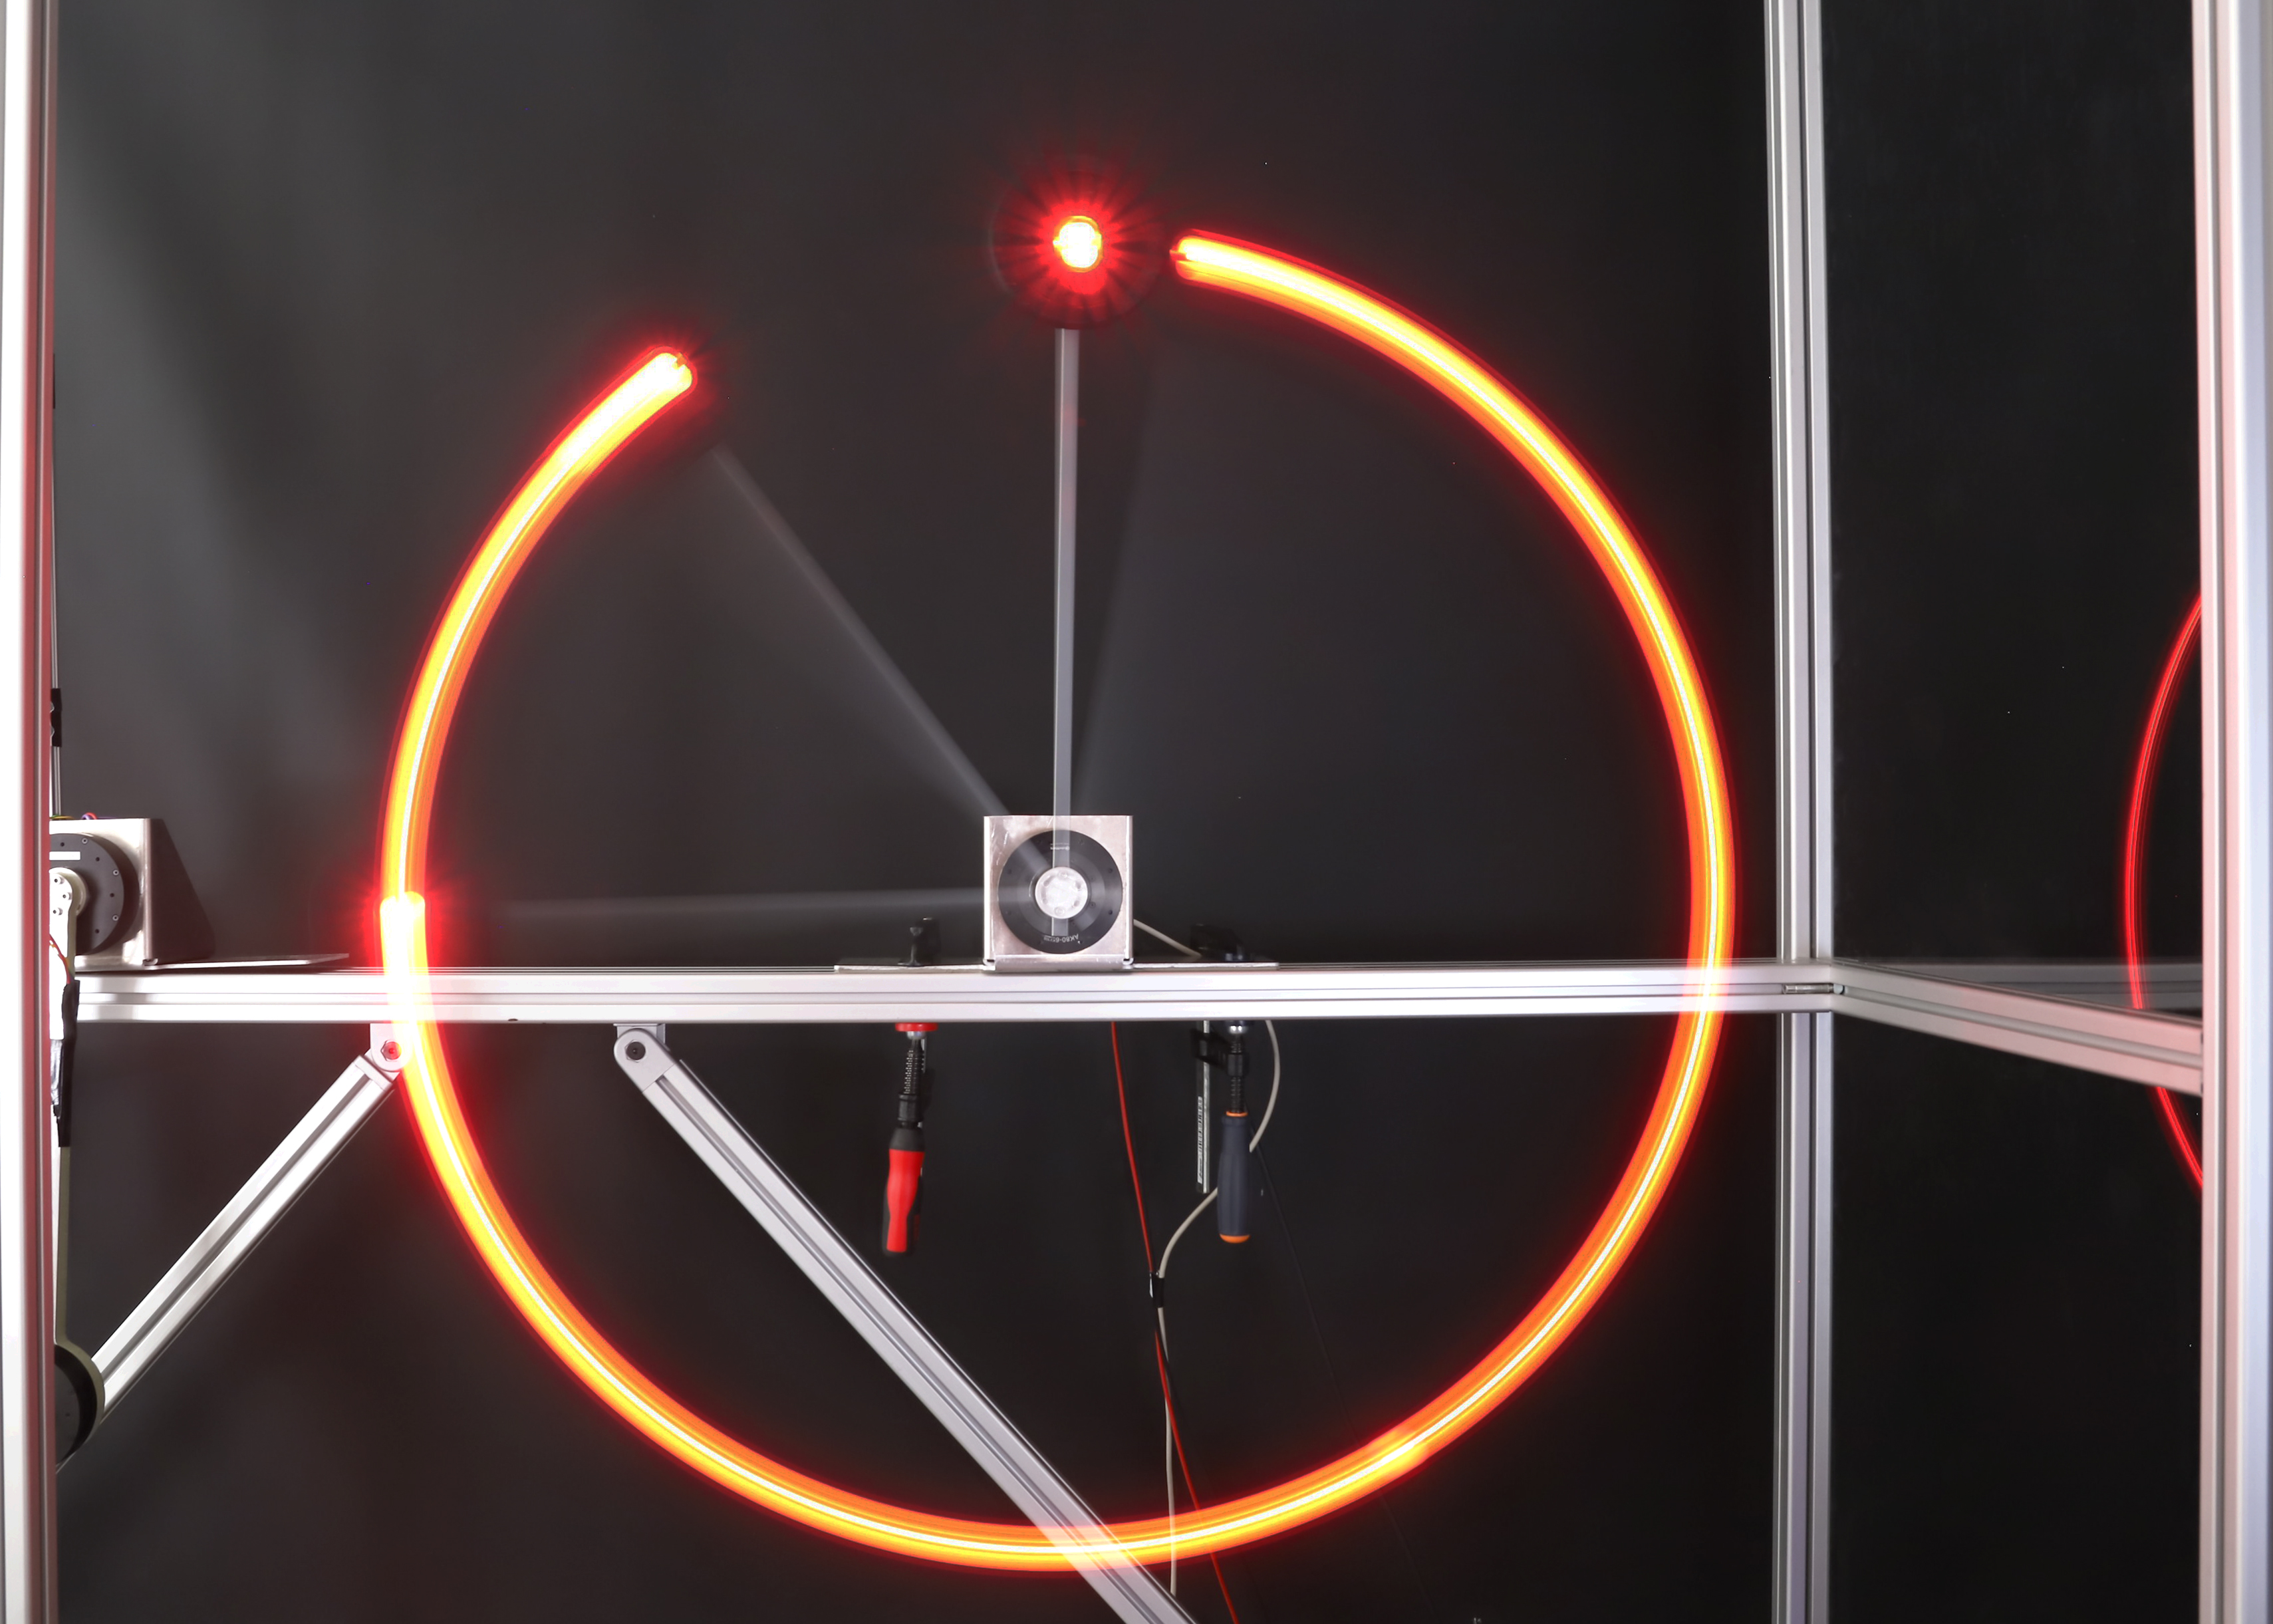
\includegraphics[width=0.4\linewidth]{figures/pendulum_light_painting.jpg}
\hspace{1 cm} 
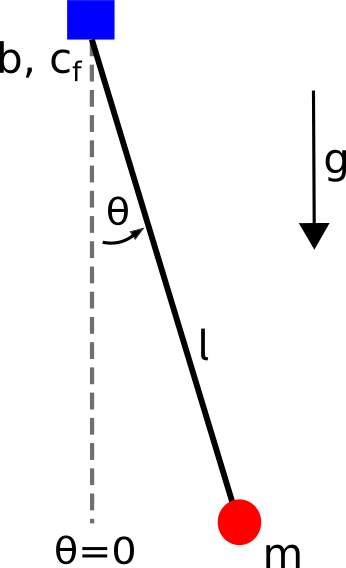
\includegraphics[width=0.2\linewidth, height = 0.28\linewidth]{figures/pendulumParams.png}
\caption{Figure 5: Simple pendulum model and real system}
\label{Pendulum parameters}
\end{figure}
\end{frame}

\begin{frame}{Open Loop Dynamics \& Phase Portrait}
\centering
\movie[autostart, loop, width=0.75\textwidth, height = 0.58\textwidth, showcontrols]{}{figures/openLoop_Pendulum.mp4}
\end{frame}

\begin{frame}{Closed Loop Dynamics \& Lyapunov Function}
\centering
\movie[autostart, loop, width=0.75\textwidth, height = 0.58\textwidth, showcontrols]{}{figures/RoA_Pendulum.mp4}
\end{frame}

\begin{frame}{Time-varying RoA Estimation}
\begin{minipage}{.4\linewidth}
\begin{block}{Time-varying features}
\begin{itemize}
  \item Region of Attraction = funnel
  \item How far can the state deviate from the nominal trajectory?
  \item More involved estimation: sampling in time, bilinear alternation, ...
\end{itemize}
\end{block}
\begin{block}{Methods}
\begin{itemize}
  \item Simulation-based approach
  \item Sum of squares(SOS) programming 
\end{itemize}
\end{block}
\end{minipage}
\begin{minipage}{.05\linewidth}
\hspace{0.1 cm}
\end{minipage}
\begin{minipage}{.48\linewidth}
\centering
\begin{figure}
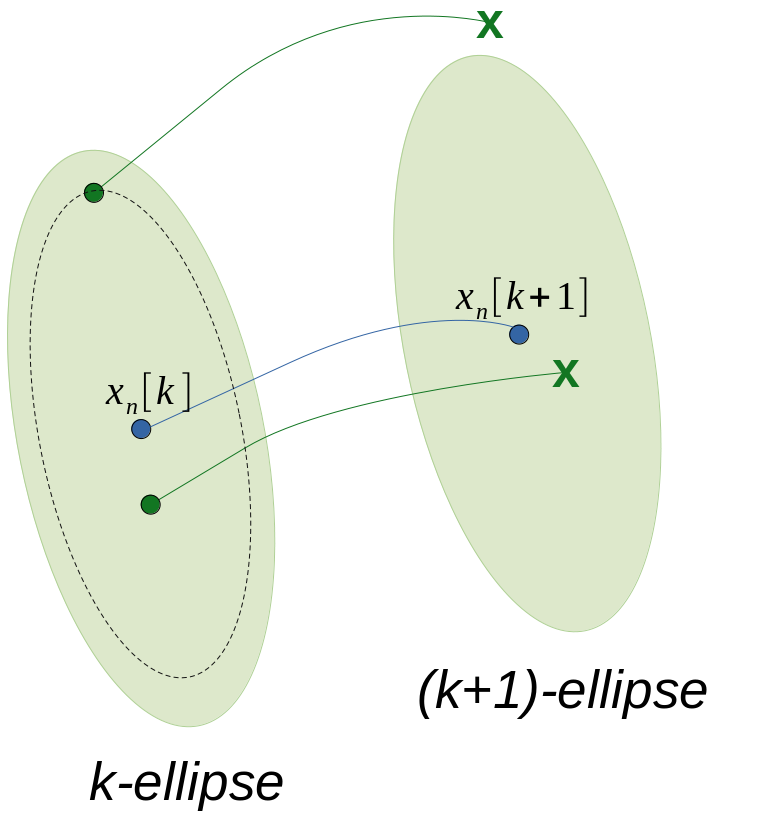
\includegraphics[width=0.5\linewidth, height=0.45\linewidth]{figures/probEllipses.png}\\
\vspace{1cm}
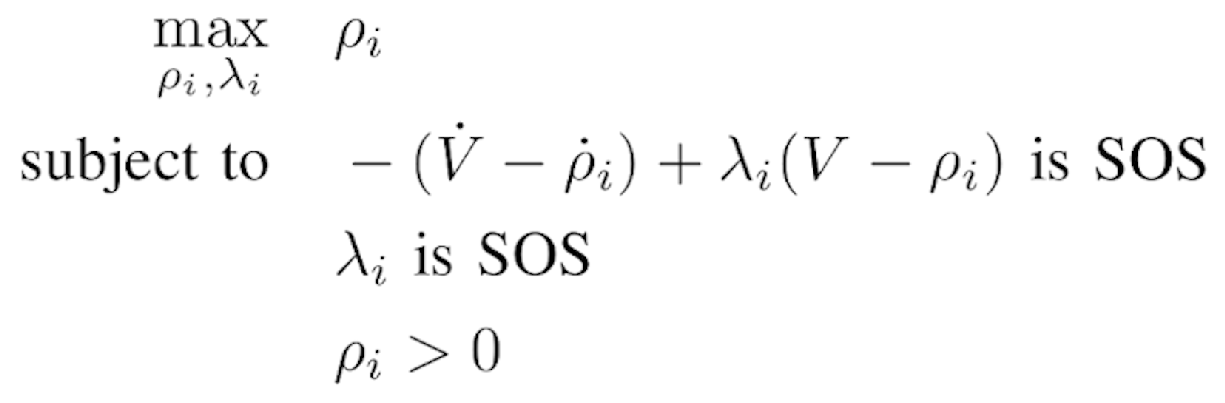
\includegraphics[width=0.8\linewidth, height=0.3\linewidth]{figures/SOSoptProblem.png}
\caption{Figure 6: RoA estimation methods}
\label{RoA Methods}
\end{figure}
\end{minipage}
\end{frame}

\begin{frame}{Pendulum: Results}
\centering
\begin{figure}
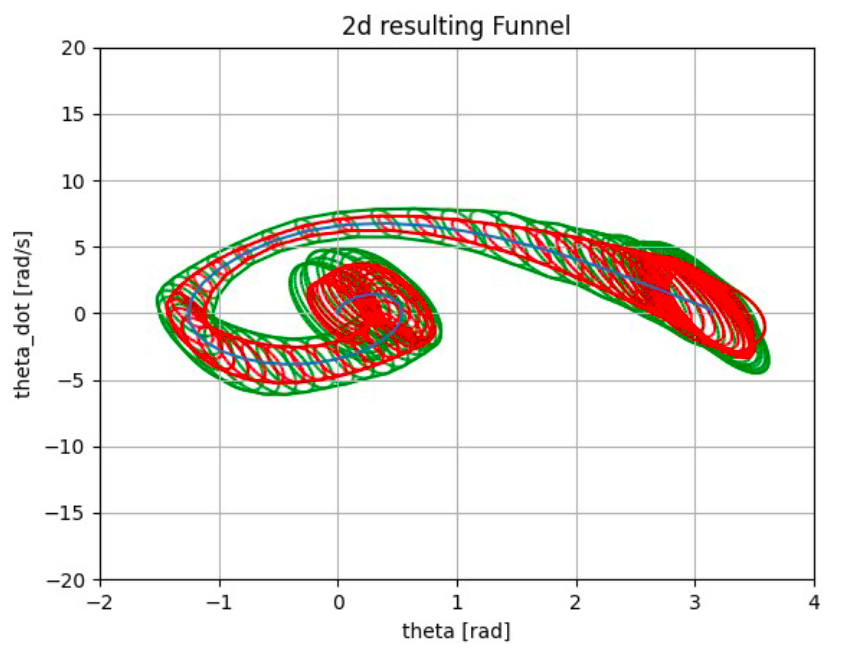
\includegraphics[width=0.5\linewidth, height=0.5\linewidth]{figures/pendulumFunnels.pdf}
\caption{Figure 7: Pendulum funnels computed via simulation-based \& SOS methods}
\label{pendulum funnel}
\end{figure}
\end{frame}

\begin{frame}{Funnel Verification}
\centering
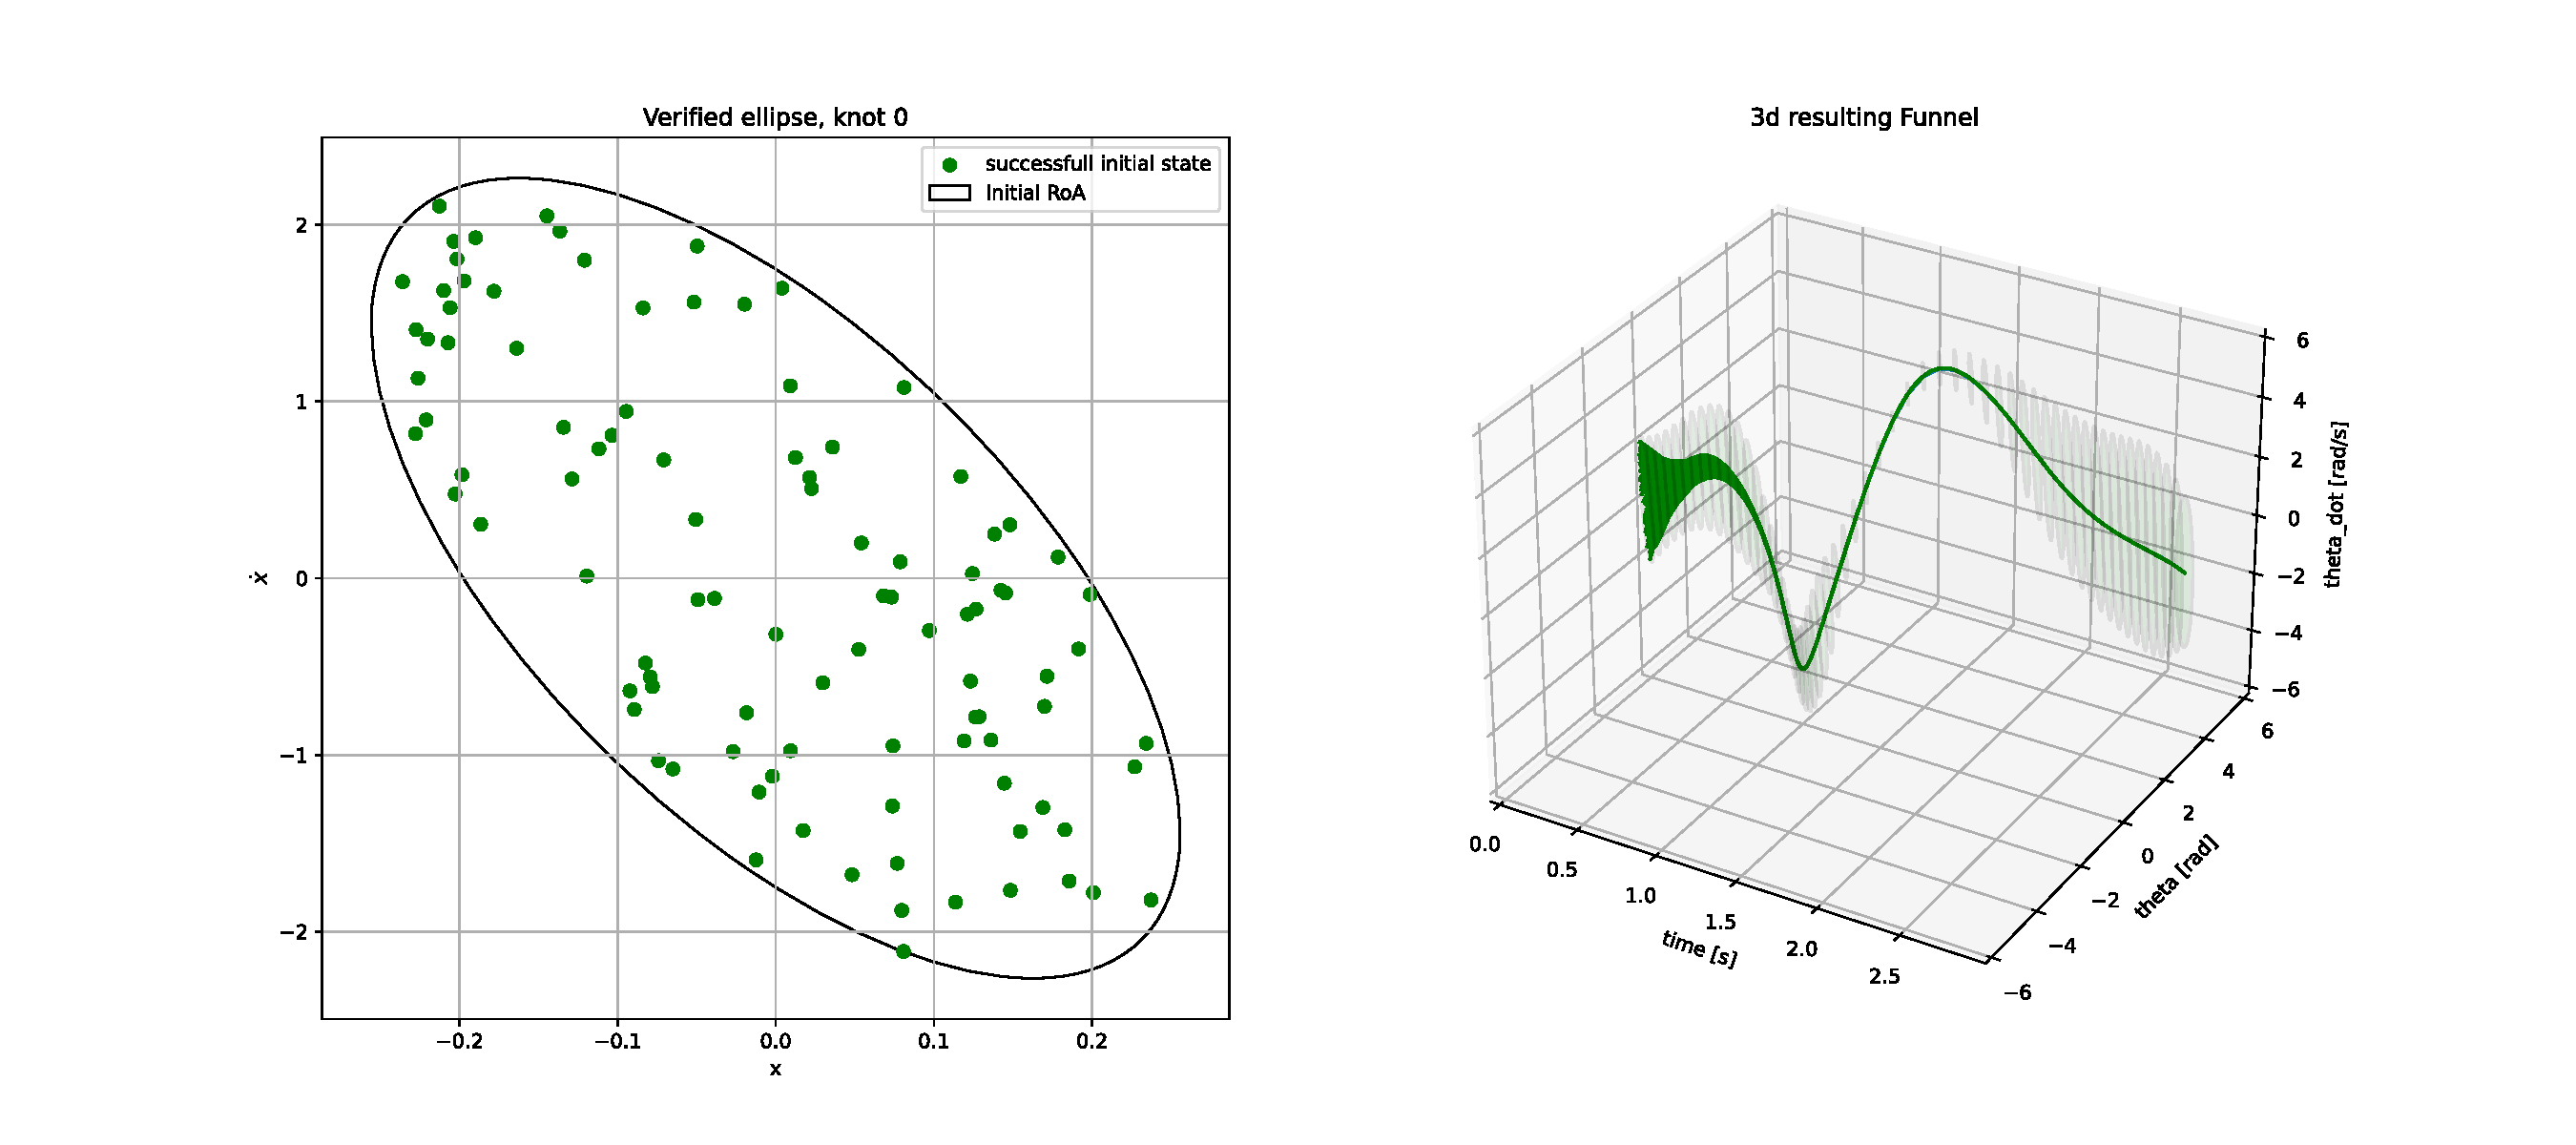
\includegraphics[width=0.9\linewidth, height=0.4\linewidth]{figures/pendulumVerify.pdf}\\
\vspace{1 cm}
Figure 8: Verification of the pendulum funnel computed via SOS
\end{frame}

\begin{frame}{Experimental Verification}
\centering
\movie[autostart, loop, width=0.45\textwidth, height = 0.58\textwidth, showcontrols]{}{figures/succInit.mp4}
\movie[autostart, loop, width=0.45\textwidth, height = 0.58\textwidth, showcontrols]{}{figures/failingInit.mp4}
\end{frame}

\section{A Robust Co-design}
\separationframe{A Robust Co-design}

\begin{frame}{The Main Components}
\begin{minipage}{.4\linewidth}
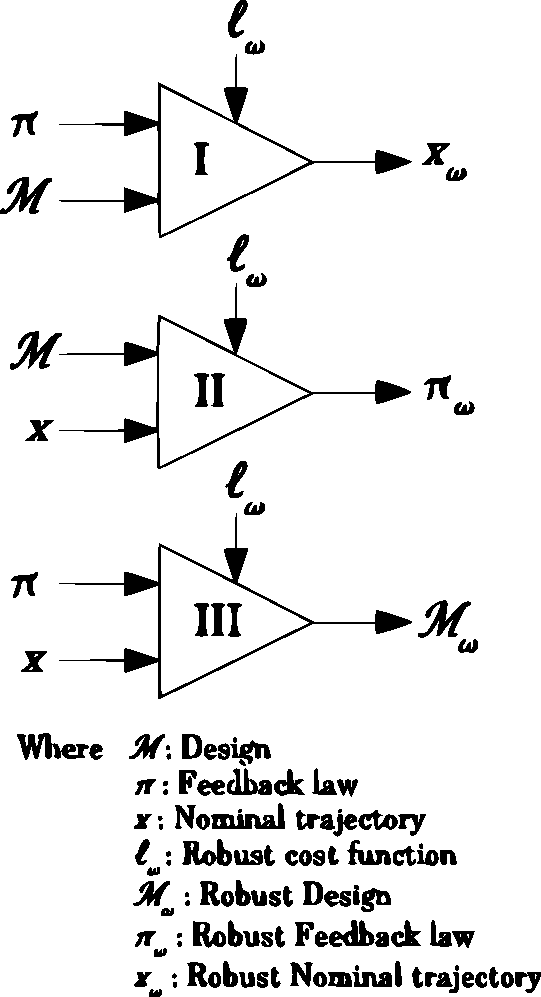
\includegraphics[width=0.7\linewidth]{figures/optBlocks.pdf}
\end{minipage}
\begin{minipage}{.45\linewidth}
\begin{block}{I: Robust trajectory optimization}
\begin{itemize}
\item Optimal trajectory to reach the goal
\item Robustness cost function
\item DIRTREL
\end{itemize}
\end{block}
\begin{block}{II: Robust trajectory stabilization}
\begin{itemize}
\item Optimal controller that stabilize a given trajectory
\item Robustness cost function
\item TVLQR
\end{itemize}
\end{block}
\begin{block}{III: Robust design optimization}
\begin{itemize}
\item Optimal design to achieve a desired state
\item Robustness cost function
\end{itemize}
\end{block}
\end{minipage}
\end{frame}

\begin{frame}{Multiple Possible Combinations}
\begin{minipage}{.4\linewidth}
\begin{block}{Robust Co-design}
\begin{itemize}
\item The order matters!
\item Iterative method (i)
\item Input variations
\end{itemize}
\end{block}
\end{minipage}
\begin{minipage}{.05\linewidth}
\hspace{0.1 cm}
\end{minipage}
\begin{minipage}{.5\linewidth}
\raggedleft
\begin{figure}
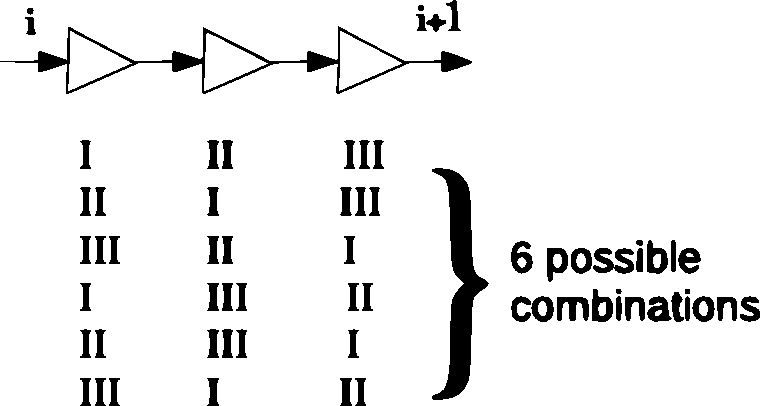
\includegraphics[width=1\linewidth]{figures/optCombinations.pdf}
\caption{Figure 9: Different possible combinations in the robust co-design}
\label{optCombinations}
\end{figure}
\end{minipage}
\end{frame}

%%%%%%%%%%%%%%%%%%%%%%%%%%%%%%%%%%%%%%%%%%%%%%%%%%%%%%%%%%%%%%%%%%%%%%%%%%%%%%%%%%%

\section{References}
\separationframe{References}

\begin{frame}{References}
\centering
\begin{minipage}{.85\linewidth}
  \begin{enumerate}[{[1]}]
    \item L. Yang et al., ''Kinematic Design Optimization of Acrobot''
    \item L. Maywald et al., ''Co-optimization of Acrobot Design and Controller for Increased Certifiable Stability''
    \item Z. Manchester and S. Kuindersma, ''DIRTREL: Robust Trajectory Optimization with Ellipsoidal Disturbances and LQR Feedback''
    \item S. Kuindersma, F. Permenter and R. Tedrake, ''An efficiently solvable quadratic program for stabilizing dynamic locomotion''
    \item S. Kuindersma, ''Recent progress on atlas, the world's most dynamic humanoid robot''
    \item E. Najafi, R. Babuska and G. Lopes, ''A fast sampling method for estimating the domain of attraction''
    \item P. Reist, P. Preiswerk and R. Tedrake, ''Feedback-motion-planning with simulation-based LQR-trees''
  \end{enumerate}
\end{minipage}
\end{frame}

\begin{frame}{References}
\centering

\begin{minipage}{.85\linewidth}
  \begin{enumerate}[{[1]}]
    \setcounter{enumi}{7}
    \item M. Tobenkin, I. Manchester and R. Tedrake, ''Invariant Funnels around Trajectories using Sum-of-Squares Programming''
    \item A. Majumdar, A. Ahmadi and R. Tedrake, ''Control Design along Trajectories with Sums of Squares Programming''
    \item J. Moore, R. Cory and R. Tedrake, ''Robust post-stall perching with a simple fixed-wing glider using LQR-Trees''
  \end{enumerate}
\end{minipage}
\vspace{2cm}
\end{frame}

\appendix

\separationframe{Thanks for your attention}

%\separationframe{Appendix}

\end{document}
